%----------------------------------------------------------------------------------------
%	Resumen
%----------------------------------------------------------------------------------------

\newpage
\clearpage{\pagestyle{empty}\cleardoublepage}
%\doublespacing
\newpage

\pagestyle{empty}
\pagenumbering{roman}
\newpage
\chapter*{\centering \large Resumen} 
\addcontentsline{toc}{chapter}{Resumen} % si queremos que aparezca en el índice
\markboth{Resumen}{Resumen} % encabezado


%Considera los siguientes puntos:
%\begin{enumerate}
%	\item Desarrolle un único párrafo (200 a 300 palabras)
%	\item Escriba en tiempo verbal presente
%	\item El resumen debe contener información sobre:
%	\begin{itemize}
%		\item	- La justificación de la investigación
%		\item	- Los objetivos o hipótesis
%		\item	- La teoría o supuestos teóricos o metodológicos en la que se sustenta
%		\item	- El método o procedimiento realizado (de ser necesario)
%		\item	- Los resultados (de ser necesario)
%		\item	- La conclusión principal
%	\end{itemize}
%\end{enumerate}



\textcolor{blue}{[BORRADOR] Escribir resumen aquí. Pellentesque venenatis, nibh id viverra elementum, ligula nulla scelerisque quam, vel vehicula nisl elit ut lorem. Nullam mattis nunc libero, ac ornare tortor consequat nec. Suspendisse eleifend nibh id lorem consequat ornare. Nunc condimentum turpis nibh, sed ultrices massa consequat nec. Ut id magna risus. Morbi id dapibus nunc. Sed quis auctor nulla. Curabitur velit metus, aliquam sit amet velit ut, tincidunt consequat magna. [/BORRADOR]}

\newpage

\begin{myfigure}[H]
	\footnotesize\centering
	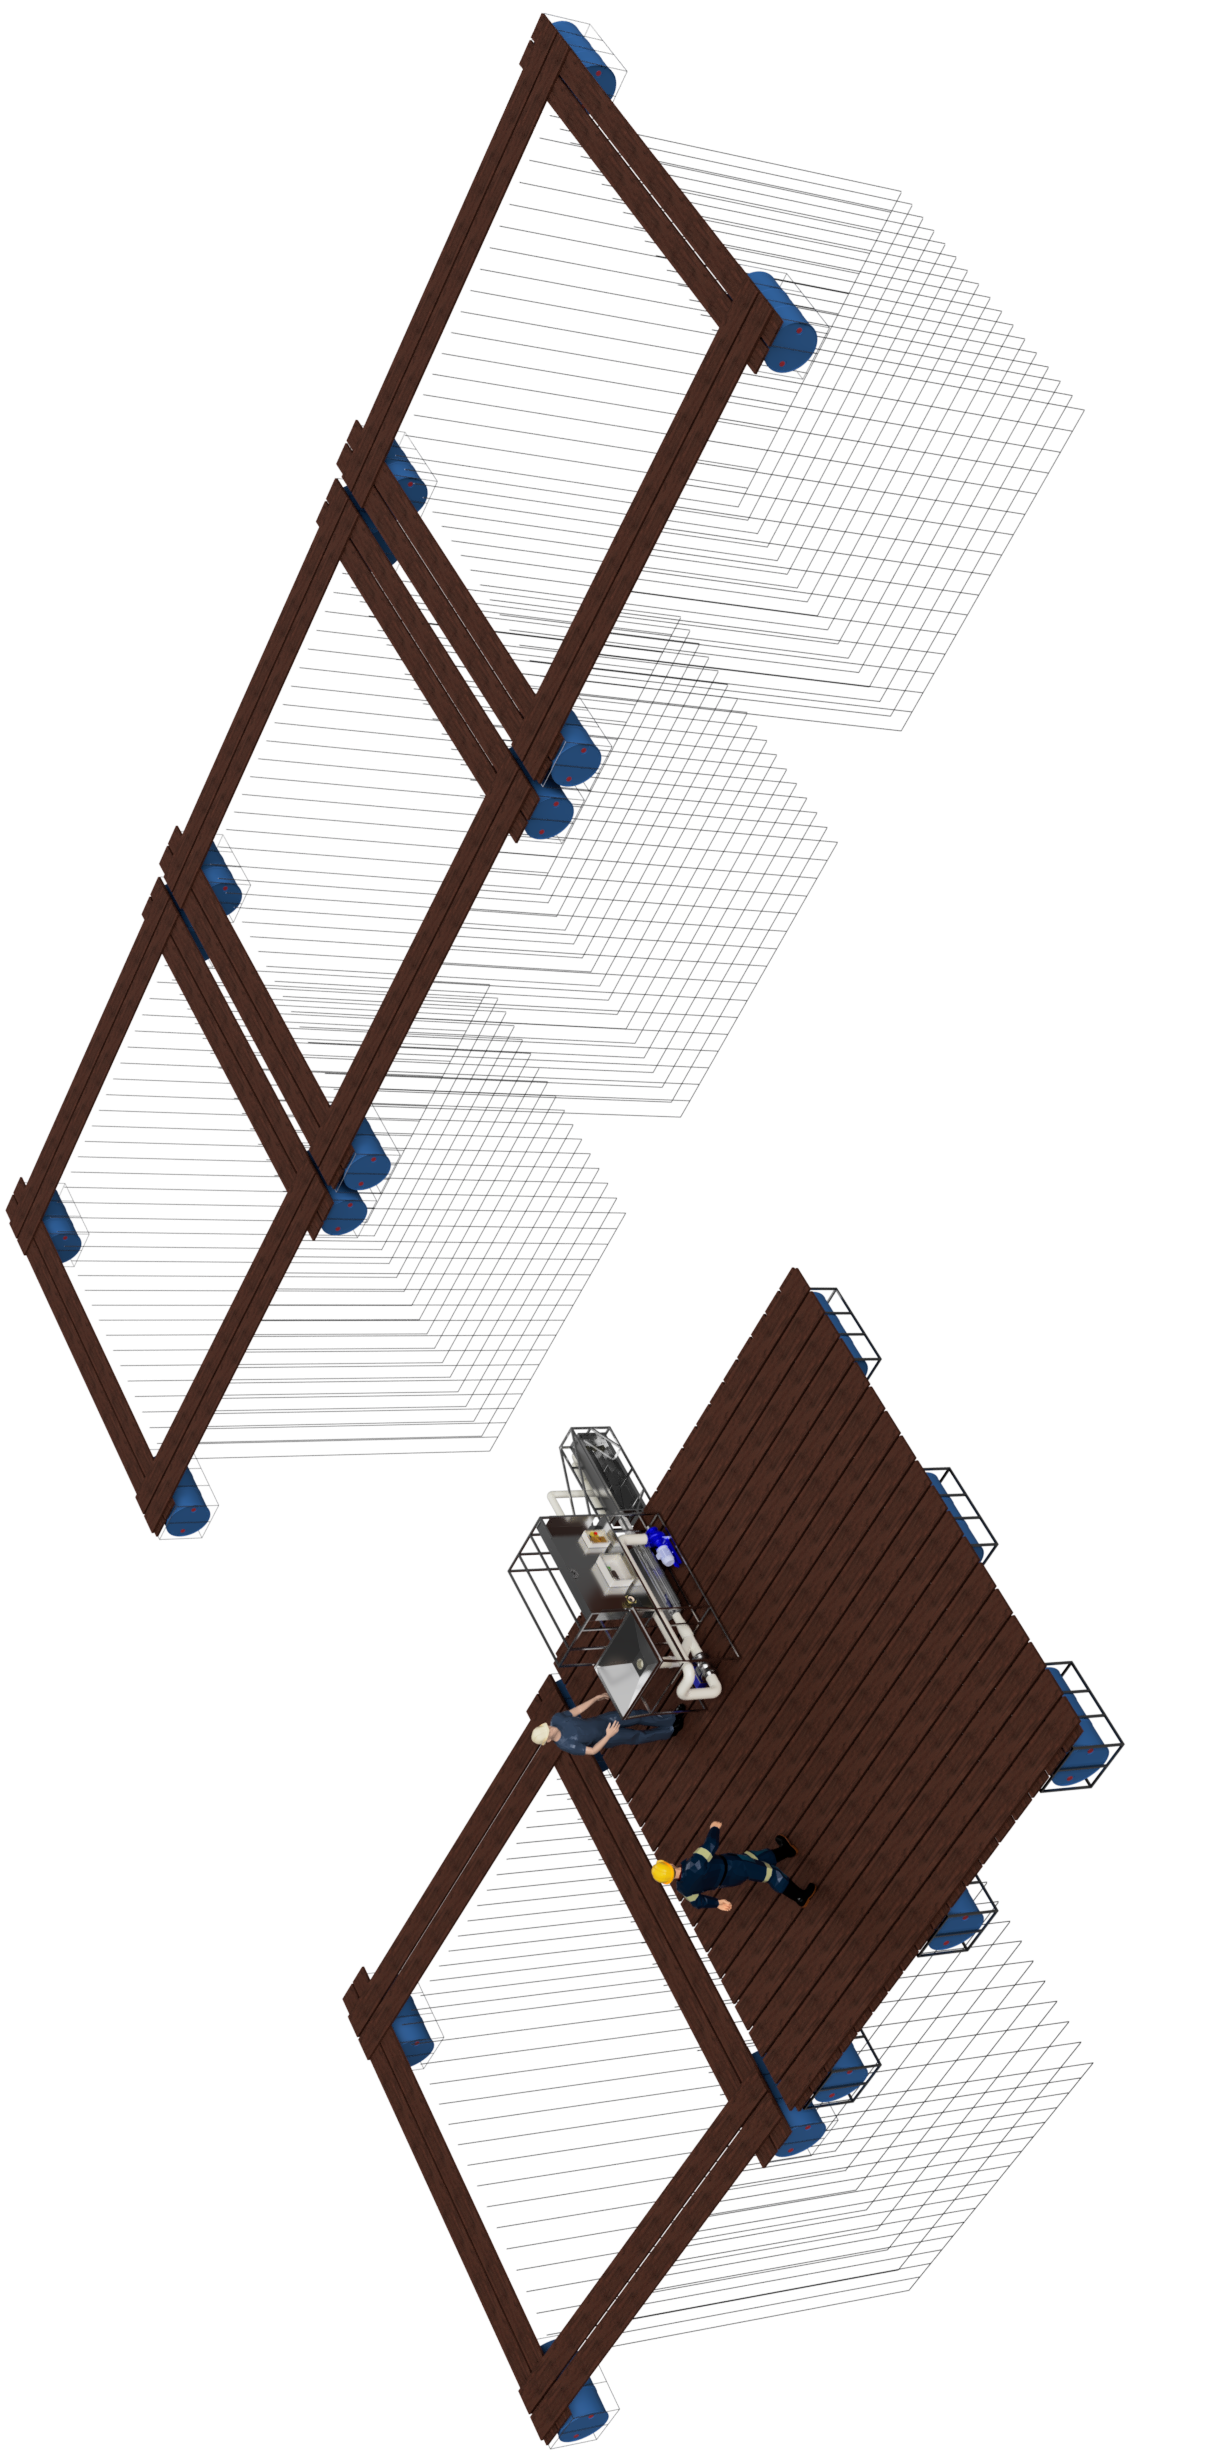
\includegraphics[width=0.80\textwidth]{total con operarios horizontal.png}
	%\caption{Diseño integral.}
	%\begin{myflushcenter}
	%	Fuente: Elaboración propia
	%\end{myflushcenter}
	%\label{fig:diseno integral}
\end{myfigure}
